\begin{figure}[htbp]
    \centering
    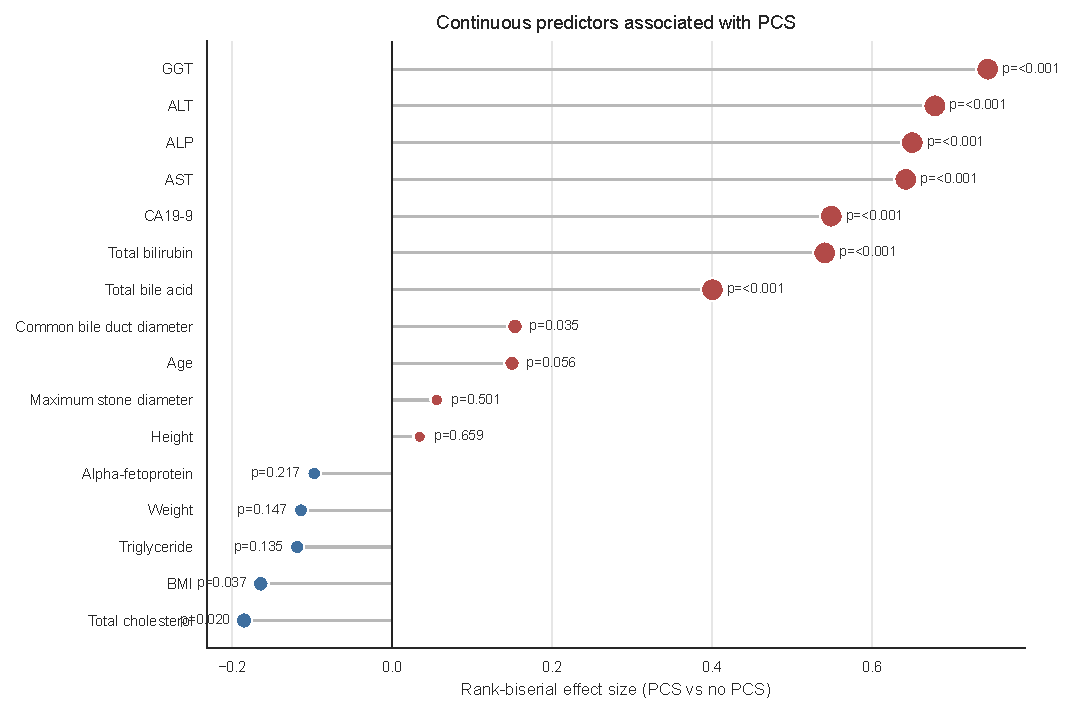
\includegraphics[width=0.92\textwidth]{output/pcs_association_figures/figure_numeric_pcs_association_lollipop.pdf}
    \caption{Univariable association between continuous predictors and PCS. Effect sizes are expressed as rank-biserial statistics from the Mann--Whitney U test, where positive values indicate higher distributions among patients with PCS. Marker size reflects the strength of statistical evidence on the $-\log_{10}(p)$ scale.}
    \label{fig:pcs_numeric_association}
\end{figure}

\begin{figure}[htbp]
    \centering
    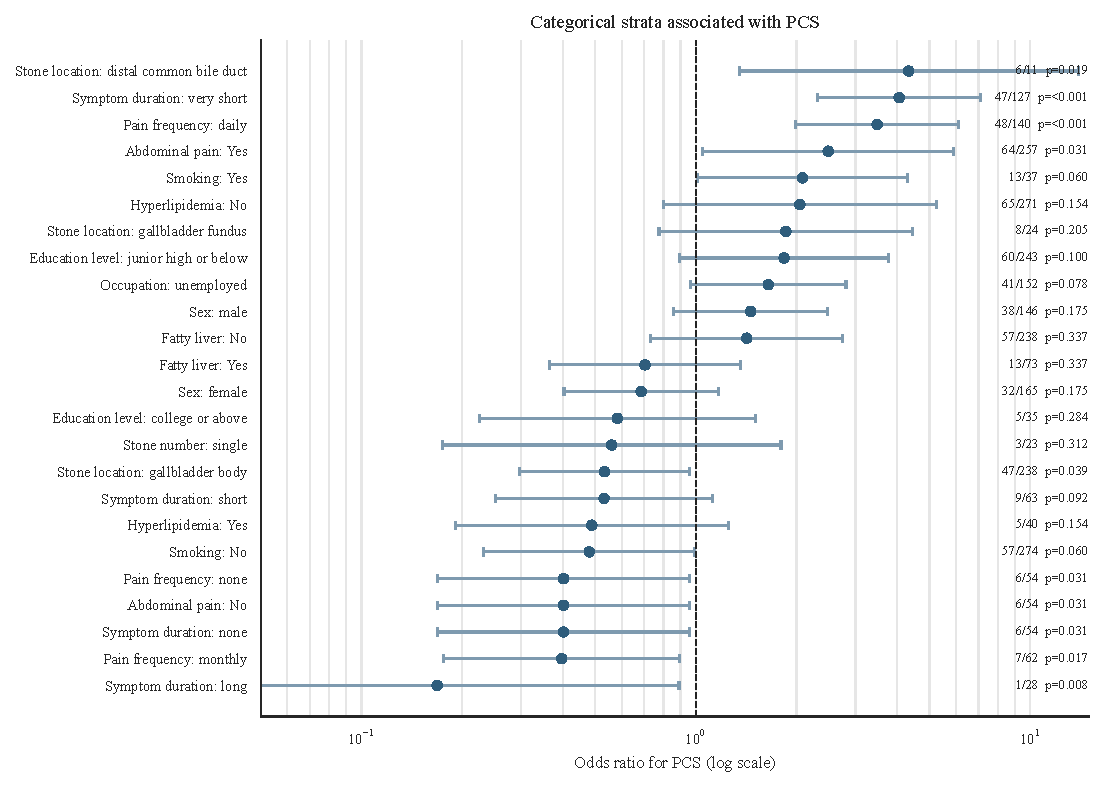
\includegraphics[width=0.92\textwidth]{output/pcs_association_figures/figure_categorical_pcs_odds_ratio_forest.pdf}
    \caption{Categorical strata associated with PCS in univariable analysis. Points denote odds ratios and horizontal bars denote 95\% confidence intervals with Haldane--Anscombe correction for sparse cells. The dashed vertical line indicates an odds ratio of 1.}
    \label{fig:pcs_categorical_forest}
\end{figure}

\begin{figure}[htbp]
    \centering
    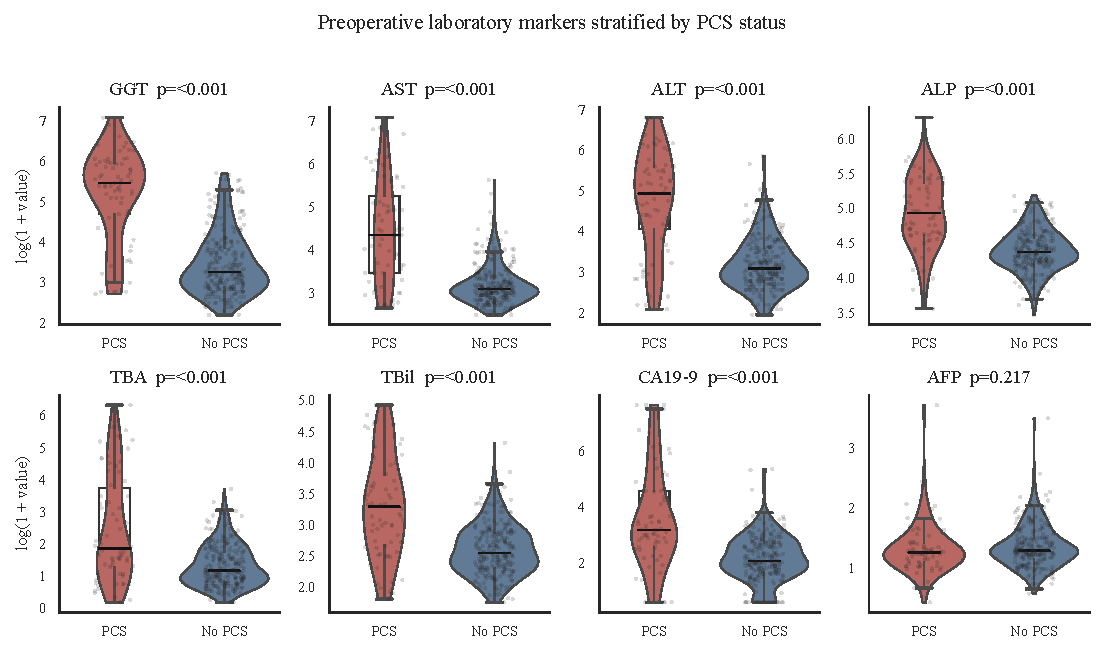
\includegraphics[width=0.92\textwidth]{output/pcs_association_figures/figure_laboratory_distributions_by_pcs.pdf}
    \caption{Distribution of selected preoperative laboratory markers stratified by PCS status. Values are displayed on a $\log(1+x)$ scale to improve visualization of skewed laboratory distributions.}
    \label{fig:pcs_laboratory_distribution}
\end{figure}

\begin{figure}[htbp]
    \centering
    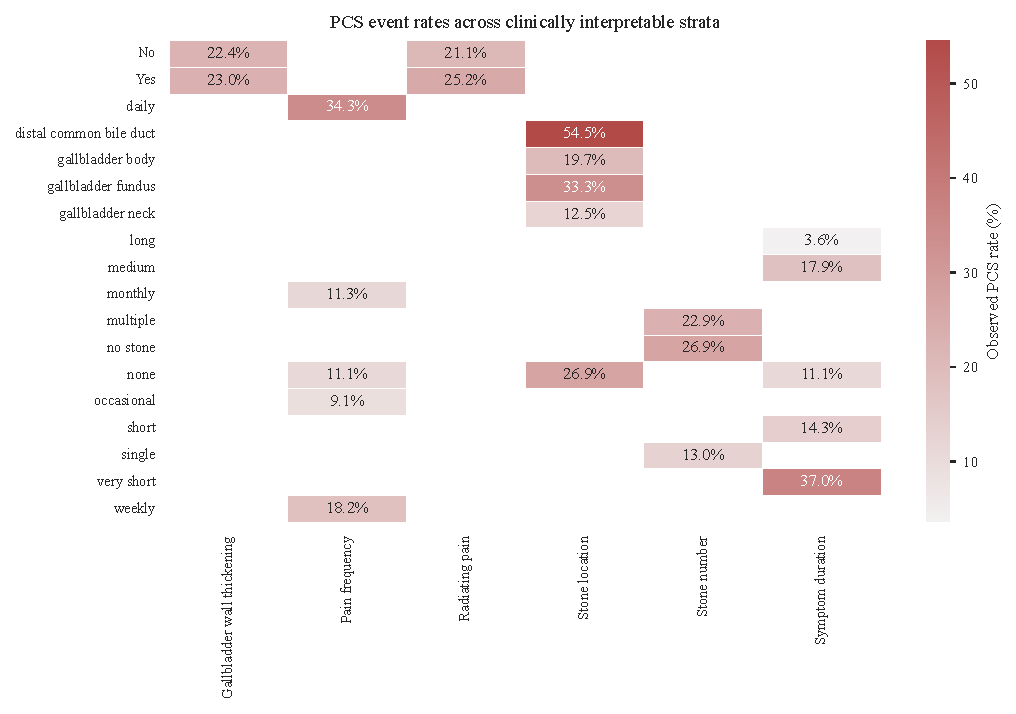
\includegraphics[width=0.92\textwidth]{output/pcs_association_figures/figure_pcs_rate_strata_heatmap.pdf}
    \caption{Observed PCS event rates across selected clinically interpretable categorical strata. Cells show the observed PCS proportion within each stratum.}
    \label{fig:pcs_rate_strata}
\end{figure}
